\documentclass{article}

\usepackage[
  paperheight=8.5in,
  paperwidth=5.5in,
  left=10mm,
  right=10mm,
  top=20mm,
  bottom=20mm]{geometry}
\usepackage[utf8]{inputenc}

\usepackage{graphicx}
\usepackage{wrapfig}
\usepackage[bottom]{footmisc}
\usepackage{listings}
\usepackage{enumitem}

\usepackage{wrapfig}
\usepackage{ragged2e}

\usepackage{array}
\usepackage[table]{xcolor}
\usepackage{multirow}
\usepackage{booktabs}
\usepackage{hhline}
\definecolor{palegreen}{rgb}{0.6,0.98,0.6}

\usepackage{amsmath}
\usepackage{amssymb}
\usepackage{multicol}
\usepackage{lipsum}
\usepackage{hyphenat}
\PassOptionsToPackage{hyphens}{url}
\usepackage{url}

\usepackage{rotating}

%\usepackage{xeCJK}

%% support use of straight quotes in code listings
\usepackage[T1]{fontenc}
\usepackage{textcomp}
\usepackage{listings}
\lstset{upquote=true}

%% for shrinking space between lines
\usepackage{setspace}

\newcommand*{\affaddr}[1]{#1} % No op here. Customize it for different styles.
\newcommand*{\affmark}[1][*]{\textsuperscript{#1}}
\newcommand*{\email}[1]{\small{\texttt{#1}}}
\newcommand{\tarot}{\textsc{Tarot}}
\renewcommand*\contentsname{\centering Table of Contents}

\renewcommand{\footnoterule}{%
  \kern -3pt
  \hrule width \textwidth height 0.5pt
  \kern 2pt
}

% remove date
\date{}

\usepackage{titlesec}
\titleformat*{\section}{\large\bfseries}
\titleformat*{\subsection}{\normalsize\bfseries}
\titleformat*{\subsubsection}{\normalsize\bfseries}

\usepackage{biblatex}


\addbibresource{references.bib}

\title{
Computer Science in the Chemistry Lab: An Interdisciplinary Project Involving Arduino-Based Temperature Sensors\footnote{\protectCopyright \copyright 2023 by the Consortium for Computing Sciences in Colleges.
Permission to copy without fee all or part of this material is granted provided
that the copies are not made or distributed for direct commercial advantage,
the CCSC copyright notice and the title of the publication and its date appear,
and notice is given that copying is by permission of the Consortium for
Computing Sciences in Colleges.  To copy otherwise, or to republish, requires
a fee and/or specific permission.
}
}

%\begin{lstlisting}
  \author{
    Brad Bauer\affmark[1], Mark Gilder\affmark[2], and Judith O'Rourke\affmark[2]\\
    \affmark[1]Department of Physical and Biological Sciences\\
    \affmark[2]Computer Science Department\\
    The College of Saint Rose\\
    Albany, NY 12203\\
    \email{\{bauerb,gilderm,orourkej\}@strose.edu}
  }
%\end{lstlisting}

\begin{document}
\maketitle

\begin{abstract}
An interactive activity was developed to connect computer science and chemistry students, 
allowing both groups to appreciate the applications of computer science to cross-disciplinary fields.  
Computer science majors are tasked with developing an Arduino system to collect and manage thermal 
data generated during laboratory experiments.  Computer science students must employ a range of techniques …. 
Once the system is complete, computer science students work alongside chemistry students to implement their 
program within an introductory chemistry experiment. %s for introductory and upper-level chemistry courses.   
Aside from the collection, 
storage, and visualization of laboratory data, chemistry students benefit by gaining experience managing large data sets and 
an %understanding and 
appreciation for computer science and its increasing value in the natural sciences.
%role in the natural sciences. %the computer science that underlies much of the laboratory equipment they use.  
%will use in college and in their careers. 
\end{abstract}


\section{Introduction}

The study of computer science is becoming necessary and fundamental to every academic discipline~\cite{columbia}.  
An understanding of computer science concepts and techniques is critical in order to analyze and 
extract meaningful information from the vast amounts of data generated in fields like biology, healthcare, 
finance, physical sciences, and mathematics.  Due to technological advancements, the ability to store and manage 
large amounts of data is easily accessible across all major STEM fields.  

Comp Sci lead-in to Arduinos as a comp sci teaching tool.  

Arduinos are also becoming increasingly common in undergraduate chemistry laboratories.  They have recently been 
utilized to develop low-cost laboratory equipment including (but not limited to) fluorometers~\cite{bullis}, 
centrifuges~\cite{sadegh}, 
pH sensors~\cite{qutieshat}, 
tensile testers~\cite{arrizabalaga}, and calorimeters~\cite{gomes}.  
In the current study, arduino systems utilizing 
thermistors are developed for use in laboratory experiments that require measurements of temperature.  

Temperature measurements provide important insight into various chemical and physical processes.  
By monitoring the variation of temperature of a sample as it is heated or cooled, characteristic 
transition temperatures such as the freezing/melting point or boiling point can be determined~\cite{atkins}.  
When considering mixtures of varying compositions, freezing point decreases proportionally to concentration.  
Analysis of freezing points over a full range of compositions from pure solvent to pure solute allows for the generation of 
two-component, solid liquid phase diagrams~\cite{martinez,blanchette}.  
Thermochemical analysis through calorimetry can also be utilized to 
determine heats of chemical reaction.  When coupled with the method of continuous variations~\cite{jobs}, stoichiometric 
ratios of chemical reactants or concentration of an unknown reactant can be determined~\cite{vernier,vonderbrink,tatsuoka,mahoney}.  
In order to capture key features in the temperature-time profiles, large numbers of data points are often collected.  
Due to the potentially large data sets generated over reasonably short time periods, prevalence in various introductory through 
advanced chemistry lab courses, and availability of inexpensive thermal probes, thermal analysis activities are a natural 
fit for this interdisciplinary project.

%The introductory chemistry laboratory experiment utilized in this activity allows students to 
%determine optimal ratios of compounds used in chemical reactions.  Students systematically vary the 
%proportions of reactants used in a chemical reaction and identify the proportion that results in 
%maximum evolution of heat (as observed through temperature changes).  



%Temperature measurements provide important insight into various chemical and physical processes.  
%By monitoring the variation of temperature of a sample as it is heated or cooled, characteristic transition 
%temperatures such as the freezing/melting point or boiling point can be determined (REF).  When considering mixtures of varying 
%compositions, freezing point decreases proportionally to concentration.  Analysis of freezing points over a full range of 
%compositions from pure solvent to pure solute allows for the generation of two-component, solid liquid phase diagrams (REF).  
%Thermochemical analysis through calorimetry can also be utilized to determine heats of chemical reaction.  When coupled with 
%the method of continuous variations (REF), stoichiometric ratios of chemical reactants or concentration of an unknown reactant 
%can be determined (REF).  In order to capture key features in the temperature-time profiles, large numbers of data points are often collected.  
%Due to the potentially large data sets generated over reasonably short time periods, prevalence in various introductory through advanced chemistry 
%lab courses, and availability of inexpensive thermal probes, thermal analysis activities are a natural fit for this interdisciplinary project.  (Support with references)

%Two chemistry laboratory activities have been identified for this activity: one in introductory courses and one in upper-level chemistry courses.  
%The first activity allows introductory students to determine optimal ratios of compounds used in chemical reactions by identifying proportions 
%that result in maximum evolution of heat as observed through temperature changes.  
%The second activity is the generation of cooling curves for mixtures of naphthalene and diphenylamine for the purpose of generating a 
%solid-liquid phase diagram.   The frequent monitoring of temperature with time using the Arduino allows chemistry students to 
%capture and identify key physical transitions (freezing points and eutectic points).  




%\section{Title and Author Information}
%Please follow the example in this paper to enter title and author information.
%The title should use title-casing. Please use \texttt{https://titlecaseconverter.com}
%with ``AP'' style to reformat your title.

%Chemistry Section 
\section{Application to Undergraduate Chemistry Laboratories}
As a proof of concept, the authors applied the thermal analysis Arduino system to an experiment currently used in an undergraduate 
General Chemistry laboratory course.  The objective of this experiment is to determine the optimal (stoichiometric) ratio of two 
reactants in a chemical reaction using the method of continuous variations~\cite{job}.  Reactants are chosen such that an 
exothermic (heat-releasing) reaction occurs; the heat released manifests as an increase in the mixture’s temperature.  
Systematically varying the ratio of these reactants and monitoring the associated temperature change ($\Delta T$) allows for the 
determination of the optimal ratio in the chemical reaction by identifying the proportion that generates the largest $\Delta T$.  
Two sets of reactants were chosen for this experiment: (1) sodium hypochlorite (NaClO) with potassium iodide (KI) and (2) NaClO with 
sodium sulfite (Na$_2$SO$_3$)~\cite{vonderbrink}.  Other combinations including 
sodium hydroxide with hydrochloric acid, 
%sodium hydroxide and 
acetic acid, 
%sodium hydroxide and 
oxalic acid,
sulfuric acid, or
phosphoric acid,
potassium hydroxide with citric acid, and sodium hypochlorite with sodium 
thiosulfate have been utilized elsewhere~\cite{mahoney,vernier,vonderbrink,tatsuoka}.

Details of the laboratory procedure can be found in Reference~\cite{vonderbink}, but 
salient details and modifications are summarized below.   0.50 M NaClO($aq$), 0.50 M KI($aq$), and 0.50 M Na$_2$SO$_3$($aq$) 
solutions were prepared.\footnote{The KI and Na$_2$SO$_3$ solutions also contained sodium hydroxide at a  0.2 M concentration.  
Details are provided in Supporting Information.}  Nine mixtures with unique ratios of each (1) NaClO solution to 
KI solution and (2) NaClO solution to Na$_2$SO$_3$ solution (by volume) were prepared such that the total volume of 
each mixture was fixed at 50.0 mL.  Components of the mixtures were kept separated until the time of the experiment.  For 
each trial, the component available in the largest volume was added to two nested Styrofoam cups and subjected to moderate magnetic stirring.  
The thermistor of the Ardunio was inserted into the liquid.  Temperature was monitored to ensure thermal equilibrium and a stable initial temperature.  
The second component was added to the first component in the cups; a button on the Arduino was pushed to record the time of mixing.  
Temperature of the resulting mixture was monitored for at least two additional minutes.  

\subsection{Determining the Optimal Ratio of the NaClO and KI Reaction}
Profiles of the observed changes in temperature with time for the reactions of NaClO and KI are shown in Figure~\ref{fig:temp_KI}.  
All temperature changes in Figure~\ref{fig:temp_KI} are expressed relative to the temperature of solution prior to mixing.  
This reference temperature for each mixture was determined as the average temperature taken over the fifteen data points prior to mixing.  
All profiles were shifted horizontally such that the time of mixing corresponds to $t = 0$ s.  Each profile is distinguished using the ratio of mL of 
NaClO($aq$) to mL of KI($aq$).

\begin{figure}[htbp]
\centering
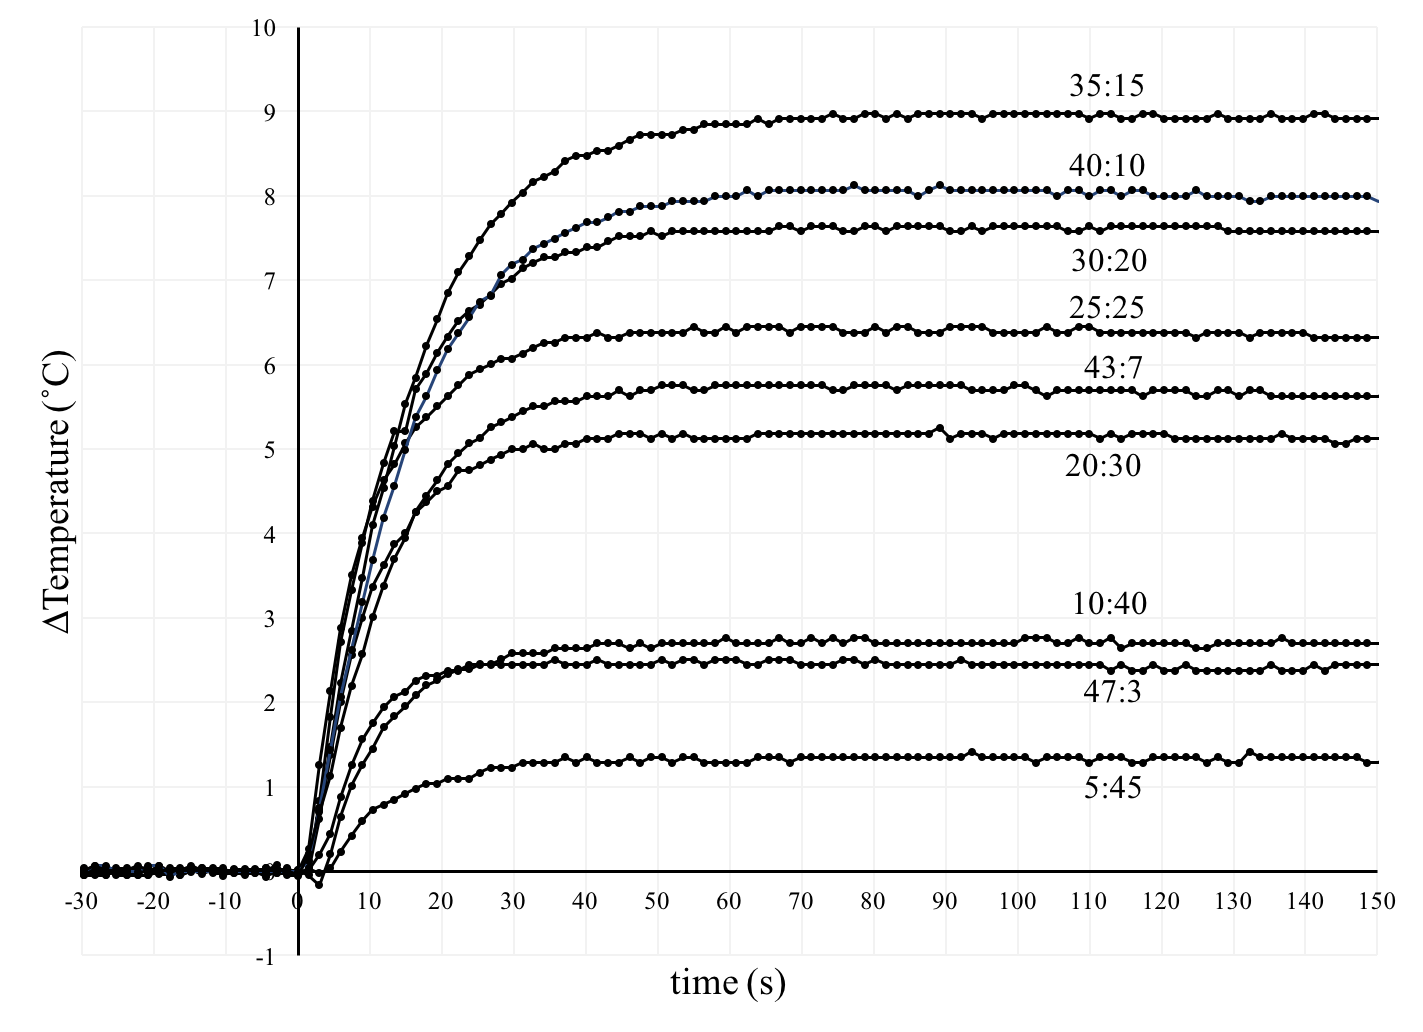
\includegraphics[width=\textwidth]{Temperature_Profiles_KI_BW.png}
\caption{Variation of Temperature with Time for Mixtures of NaClO($aq$) and KI($aq$)}
\label{fig:temp_KI}
\end{figure}


From the data sets for each trial, a maximum temperature change ($\Delta T_\mathrm{max}$) was determined.  
These $\Delta T_\mathrm{max}$ values were then plotted against the volume of NaClO solution present in the reaction 
mixture (Figure~\ref{fig:var_KI}).  In addition to the nine measured data points, two additional points 
corresponding to 0.0 mL NaClO($aq$):50.0 mL KI($aq$) and 50.0 mL NaClO($aq$):0.0 mL KI($aq$) were included.  
Since no reaction occurs at these compositions, $\Delta T_\mathrm{max}$ was taken to be 0.0$^\circ$C for these points.  
Lines of best fit through points falling on increasing and decreasing $\Delta T_\mathrm{max}$ with volume NaClO($aq$) 
trends were determined.\footnote{The upward trendline was set to include the point (0.0 mL, 0.0$^\circ$C). The downward 
trendline was set to include the point (50.0 mL, 0.0$^\circ$C). The corresponding equations were 
$\Delta T_\mathrm{max}$ = (0.2578$^\circ$C/mL) $V$ ($R^2$ = 0.99895) and $\Delta T_\mathrm{max}$ = ($-0.8169^\circ$C/mL) $V$ + 40.845$^\circ$C ($R^2$= 0.99983).}  

\begin{figure}[htbp]
\centering
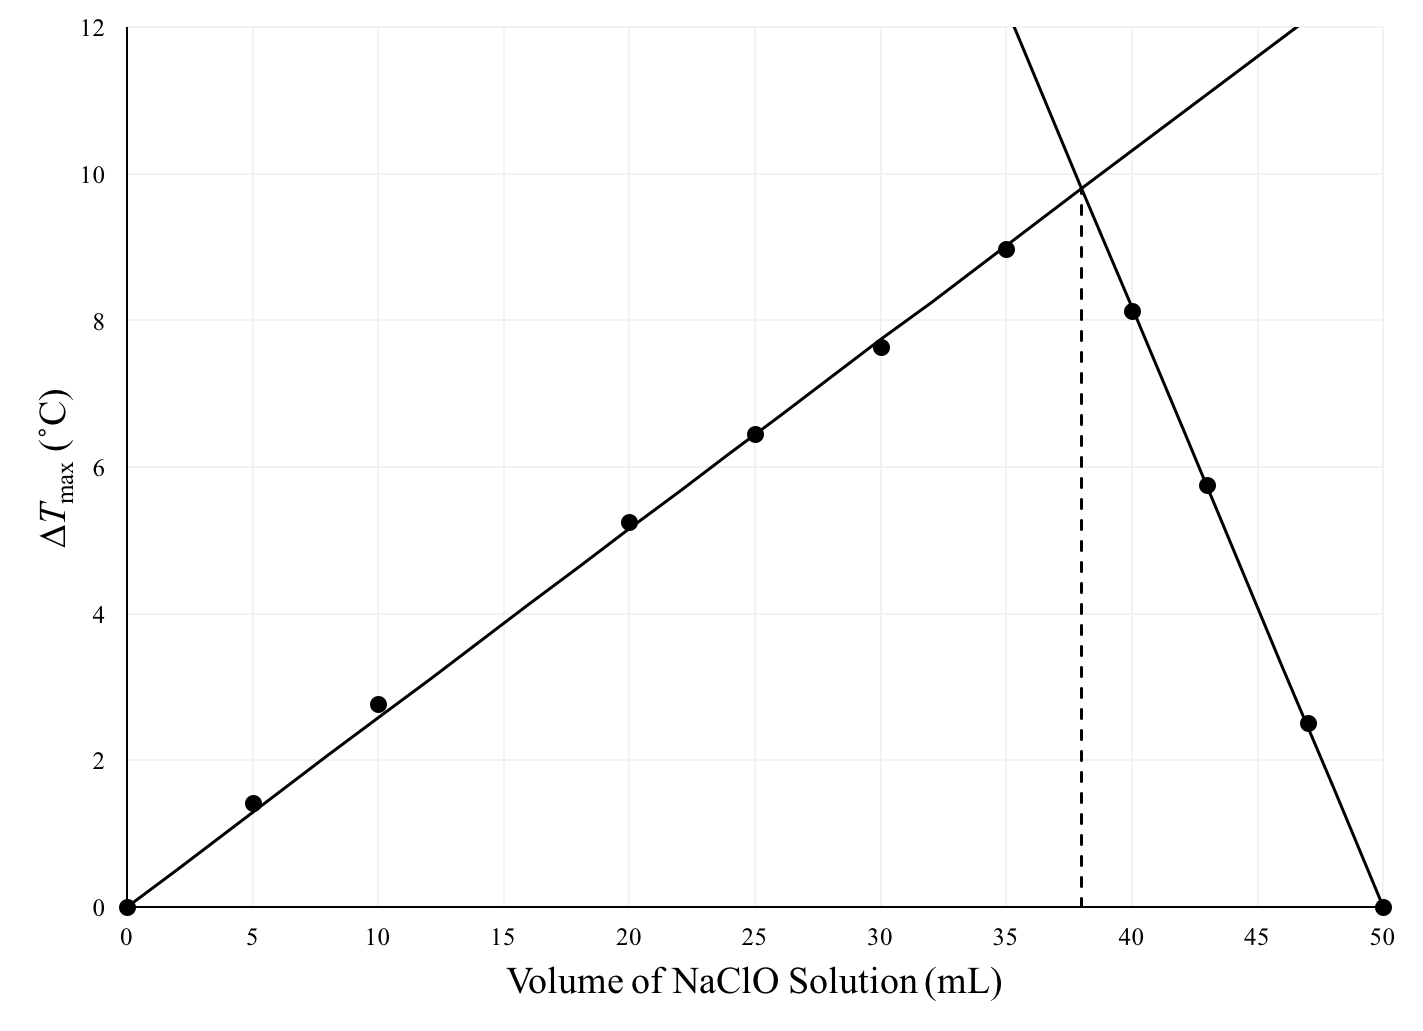
\includegraphics[width=\textwidth]{Bleach_KI_Variations_alt.png}
\caption{Maximum Temperature Changes Observed for Each Reaction Mixture of NaClO($aq$) and KI($aq$)}   %Variation of Temperature with Time for Mixtures of NaClO($aq$) and KI($aq$)}
\label{fig:var_KI}
\end{figure}

In this experimental method, the heat generated from each reaction (proportional to the $\Delta T_\mathrm{max}$ observed) 
will increase as components react more completely.  The optimal (stoichiometric) proportion of two reactants will yield the largest $\Delta T_\mathrm{max}$.  
By extrapolating the two linear trendlines to a point of intersection, we estimate the largest $\Delta T_\mathrm{max}$ to be 9.80$^\circ$C.  
This corresponds to an optimal ratio of 38.0 mL NaClO($aq$):12.0 mL KI($aq$), which is in agreement with the actual 3:1 ratio for this 
reaction.\footnote{Since solutions are at equal concentrations, the ratio of volumes is equivalent to the ratio of amounts used to establish the 
stoichiometry of the reaction.  The actual stoichiometry of 3:1 is based on the net ionic equation: 3ClO$^-$($aq$) + I$^-$($aq$) $\rightarrow$ 3Cl$^-$($aq$) + IO$_3^-$($aq$)~\cite{vonderbrink}.}

\subsection{Determining the Optimal Ratio of the NaClO and Na$_2$SO$_3$ Reaction}
The experiment was repeated using sodium hypochlorite (NaClO) with %a different reactant, 
sodium sulfite (Na$_2$SO$_3$).  
Temperature versus time plots for the NaClO and Na$_2$SO$_3$ reactions are shown in Figure~\ref{fig:temp_Na2SO3}.  
All temperature changes are expressed relative to the pre-mixing temperature and times are expressed relative to 
the time of mixing, as discussed previously.  

\begin{figure}[htbp]
\centering
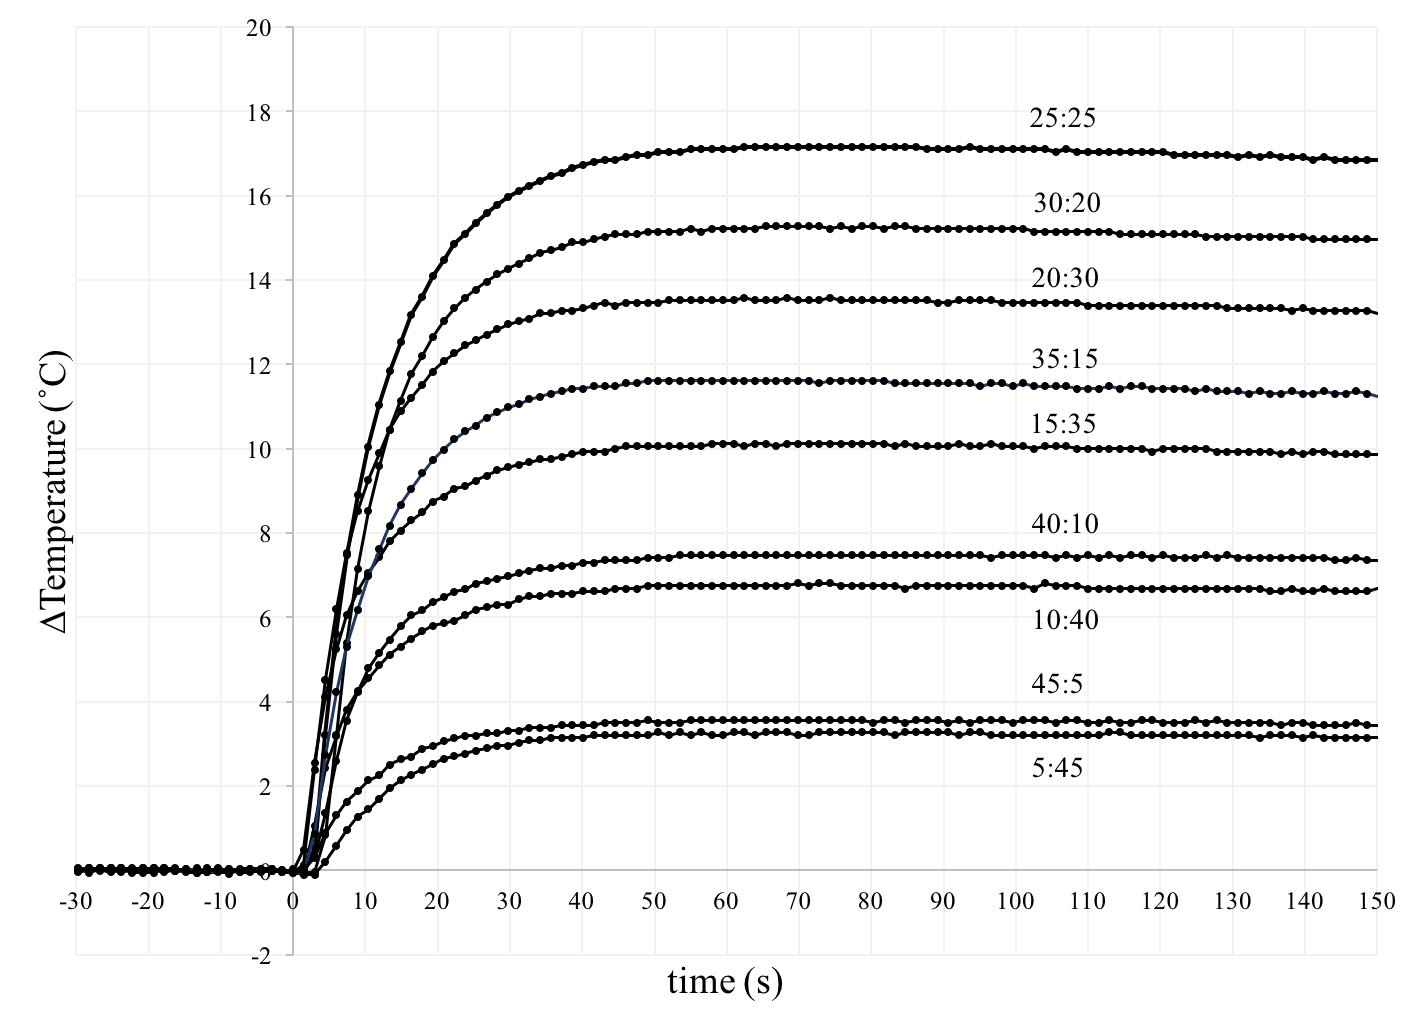
\includegraphics[width=\textwidth]{Temperature_Profiles_Na2SO3_BW.png}
\caption{Variation of Temperature with Time for Mixtures of NaClO($aq$) and Na$_2$SO$_3$($aq$)}
\label{fig:temp_Na2SO3}
\end{figure}

The maximum $\Delta T$ for each mixture was recorded and plotted 
against the volume of NaClO($aq$) in the mixture; these results are shown in Figure~\ref{fig:var_Na2SO3}.  
Points corresponding to 0.0 mL NaClO($aq$):50.0 mL Na$_2$SO$_3$($aq$) and 50.0 mL NaClO($aq$):0.0 mL Na$_2$SO$_3$($aq$) 
(each with $\Delta T_\mathrm{max} = 0.0^\circ$C) were included.  Lines of best fit were generated through each the upward and downward 
trends.\footnote{The point corresponding to 25.0 mL NaClO($aq$):25.0 mL Na$_2$SO$_3$($aq$) was included in the upward trend.  
As before, the lines were forced through the end points.  The resulting equations of the lines of best fit 
are: $\Delta T_\mathrm{max}$ = (0.6813$^\circ$C/mL) $V$ ($R^2$ = 0.99977) and $\Delta T_\mathrm{max}$ = ($-0.7629^\circ$C/mL) $V$ + 38.145$^\circ$C ($R^2$= 0.99923).}  
The intersection of these lines occurs at 26.4 mL NaClO($aq$) and $\Delta T_\mathrm{max} = 18.0^\circ$C.  This 
corresponds to a predicted optimal ratio of 26.4 mL NaClO($aq$) to 23.6 mL Na$_2$SO$_3$ (simplified to 1.12:1), 
which is in agreement with the predicted stoichiometry of 1:1.\footnote{The actual stoichiometry of 1:1 is 
based on the net ionic equation: ClO$^-$($aq$) + SO$_3^{2-}$($aq$) $\rightarrow$ Cl$^-$($aq$) + SO$_4^{2-}$($aq$)~\cite{vonderbrink}.}

\begin{figure}[htbp]
\centering
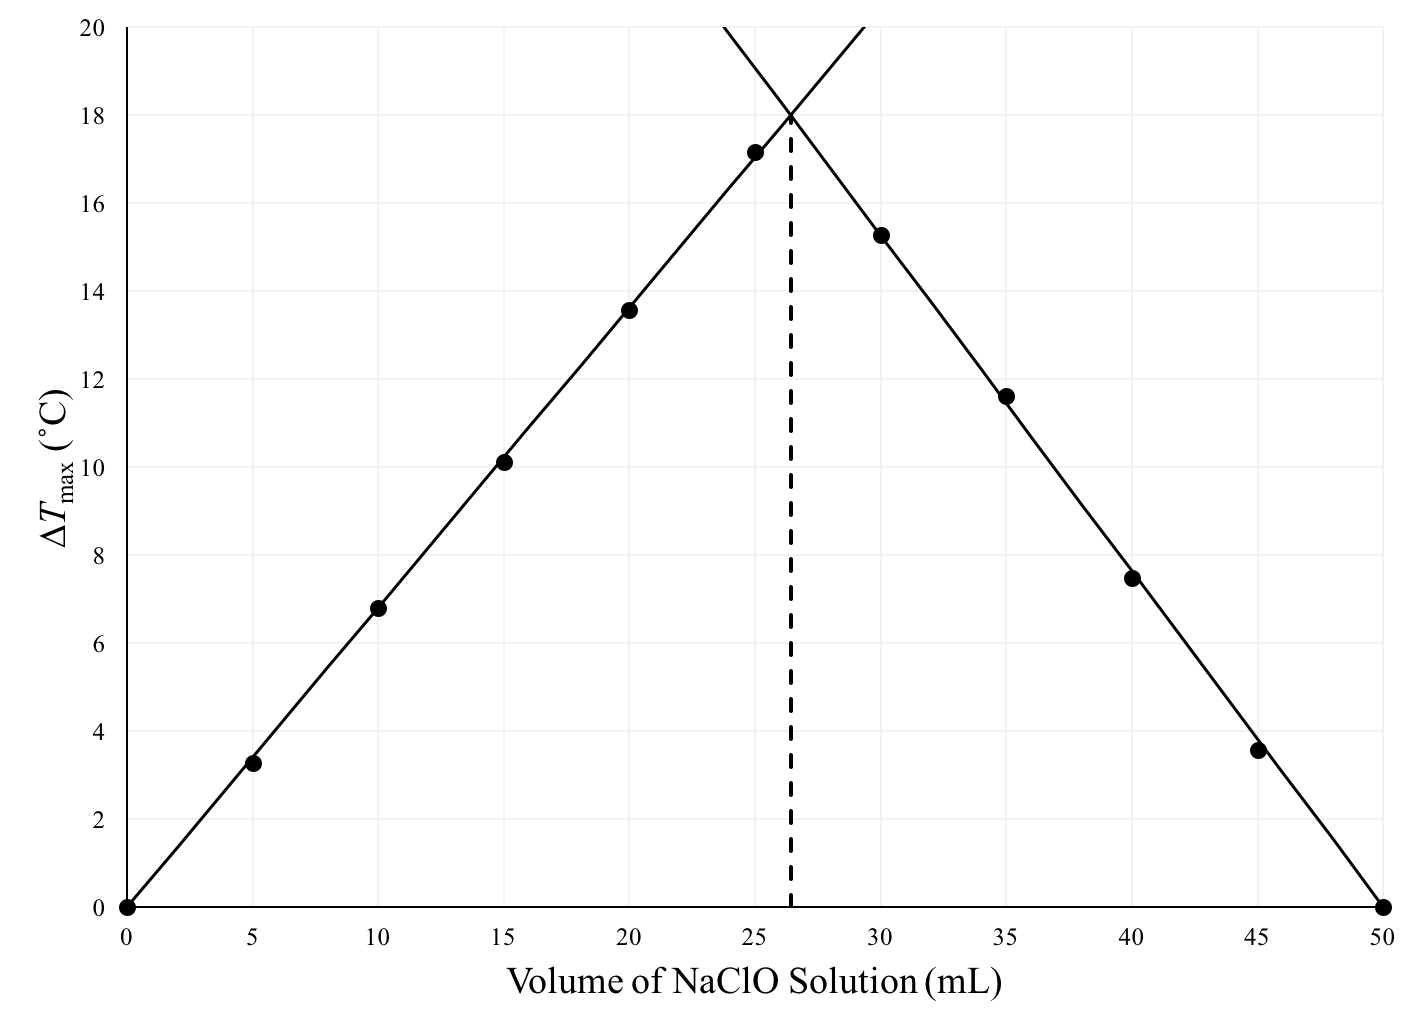
\includegraphics[width=\textwidth]{Bleach_Na2SO3_Variations.png}
\caption{Maximum Temperature Changes Observed for Each Reaction Mixture of NaClO($aq$) and Na$_2$SO$_3$($aq$)}   %Variation of Temperature with Time for Mixtures of NaClO($aq$) and KI($aq$)}
\label{fig:var_Na2SO3}
\end{figure}

\subsection{Improving the Accuracy of Results}
The method employed above allows students to quickly and easily determine the stoichiometric ratio in a chemical reaction with minimal calculations.  
The determined ratios of 3.17:1 (NaClO:KI) and 1.12:1 NaClO:Na$_2$SO$_3$ were of sufficient accuracy to conclude the correct ratios of 3:1 and 1:1 when 
rounded to the nearest whole number.  The accuracy of these ratios can be improved using some post-lab corrections.  One notable correction involves the 
adjustment of the initial temperature.  Initial temperature was determined using only the component in the mixture with the largest volume; this 
assumes that both reactants are at this initial temperature.  If the components are at different initial temperatures, a weighted average can be 
utilized~\cite{vonderbrink} to determine a more representative initial temperature as:
\begin{displaymath}
T_{i,\mathrm{avg}} = \left(\frac{V_\mathrm{A}}{V}\right)T_{i,\mathrm{A}} + \left(\frac{V_\mathrm{B}}{V}\right)T_{i,\mathrm{B}}
\end{displaymath}
where $V_\mathrm{A}$ and $V_\mathrm{B}$ represent the volumes of components A and B in the mixture, $V$ represents the total volume of the mixture, 
and $T_{i,\mathrm{A}}$ and $T_{i,\mathrm{B}}$ represent the initial temperatures of components A and B.\footnote{In order to apply this correction, 
an additional measurement of the initial temperature of the minor component must be obtained using a separate thermometer.}  This temperature 
correction was applied to the NaClO/Na$_2$SO$_3$ reactions; results are shown in Figure~\ref{fig:var_Na2SO3_corr}.\footnote{When conducting the 
experiment using these reactants, initial temperatures varied by as much as 2$^\circ$C.  Initial temperature variations for the NaClO/KI reactions 
were less significant at approximately $0.5^\circ$C.} 

\begin{figure}[htbp]
\centering
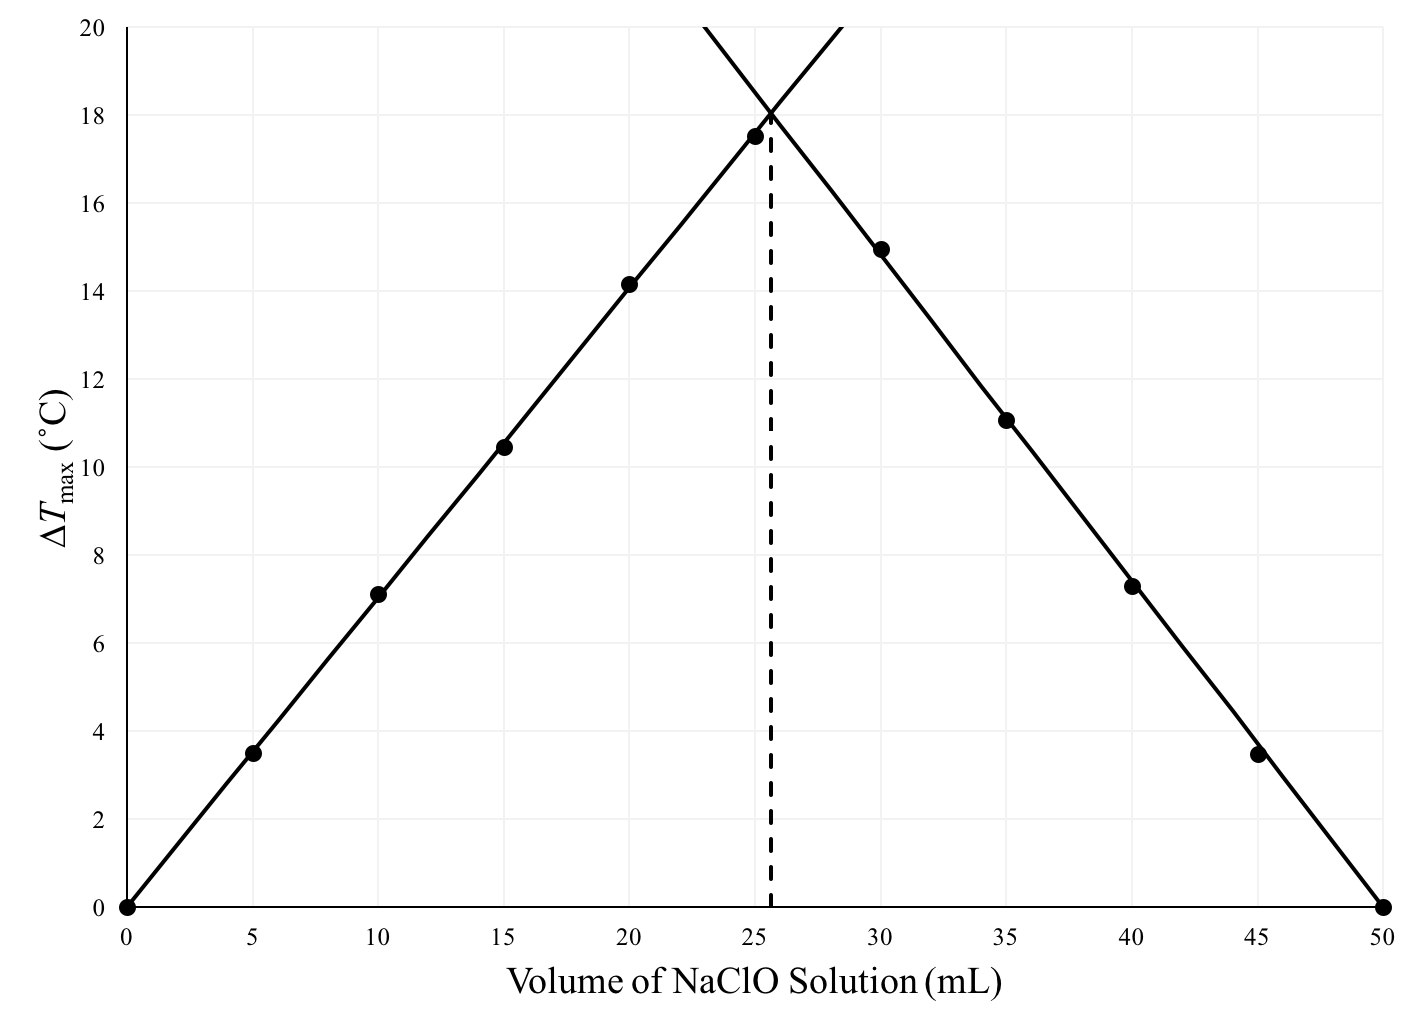
\includegraphics[width=\textwidth]{Bleach_Na2SO3_Variations_Corrected.png}
\caption{Maximum Temperature Changes for Mixtures of NaClO($aq$) and Na$_2$SO$_3$($aq$) with Initial Temperature Correction}   %Variation of Temperature with Time for Mixtures of NaClO($aq$) and KI($aq$)}
\label{fig:var_Na2SO3_corr}
\end{figure}

The corrected data yield a more accurate ratio of 25.6 mL NaClO(aq) to 24.4 mL Na$_2$SO$_3$($aq$), 
which simplifies to 1.05:1.  The observed variations are also more symmetric about the intersection composition, as is expected for a 1:1 ratio.  

The method used assumes equal concentrations of the reactants.  Slight differences in concentrations may lead to deviations from the true ratios.  
Concentrations can be incorporated using the expression
\begin{displaymath}
\mathrm{Ratio} = \frac{n_\mathrm{A}}{n_\mathrm{B}} = \frac{M_\mathrm{A}V_\mathrm{A}}{M_\mathrm{B}V_\mathrm{B}}
\end{displaymath}
where $M$ represents the molar concentration of component A or B, $V$ represents the volume of A or B at the optimal ratio, and $n$ indicates the amount
of the component A or B at the optimal ratio.  
This can be an important correction if the NaClO($aq$) solution was prepared from an older bleach solution, as some decomposition is possible.  An accurate 
concentration of NaClO($aq$) can be determined through titration analysis~\cite{vonderbrink}.  




%\subsection{Citation}
%Appropriately cite all references to other published works included in the paper.
%\texttt{biblatex} is used to create a list of references or bibliography as the
%last section in the paper. Here are citation examples for a
%book\cite{latexcompanion}, a journal paper\cite{einstein}, a
%website\cite{knuthwebsite}, and a conference proceeding paper\cite{maurer}.
%Please check out the source code of this document for details.

%\subsection{Double Quote}
%The proper way to typeset double quote is to use two backticks or grave accents
%(\`{}) on the left and two single quotes (\'{}) on the right, e.g.
%\`{}\`{}Hello!\'{}\'{} for ``Hello!''.

\subsection{Reference List}
The \verb+\printbibliography+ command prints a list of references for you.
Please use \texttt{sample.bib} as an example to create your bibliography entries.

%If you can find a reference on \url{https://scholar.google.com/} you can get a
%``BibTex'' export by clicking on the quotation mark symbol, which is a lot easier
%than entering the information manually.

%\subsection{Code Listings}
%Commands from \texttt{listings} package allow you to display code easily with
%customizable coloring and styling rules. Here is an example.
%Please check out the source code of this document for details.

%\begin{lstlisting}[language=Python,  caption=Python example]
%x = 42
%epsilon = 0.01
%step = epsilon**2
%num_guesses = 0
%ans = 0.0
%while abs(ans**2-x) > epsilon and ans < x:
%    ans = ans + step
%    num_guesses += 1
%if abs(ans**2-x) <= epsilon:
%    print(str(ans) +
%    ' is close to the square root of ' +
%    str(x))
%else:
%    print('Failed to find square root of ' + str(x))
%print("The number of guesses is " + str(num_guesses))
%\end{lstlisting}

%\section{Manuscript Submission}
%The following materials will need to be submitted:
%\begin{enumerate}[noitemsep]
%  \item The final manuscript in Latex.
%  \item Copyright release. It is essential that we receive the copyright
%  release form. By signing this form you are acknowledging that the manuscript
%  has not been printed in another venue, plus you are retaining your rights for
%  use of the manuscript. Read the copyright release. The Consortium will not
%  prohibit you from using the manuscript, but will ask that you credit any reuse
%  to the Consortium as the original source of publication. If you misplace the
%  copyright form, a generic copyright form can be found through the Copyright
%  Release Form\cite{copyright}.\\
%  The Consortium encourages multiple presentations of tutorials and workshops.
%  If you are presenting a tutorial or workshop you may retain the copyright,
%  but we must have that documented. Keep in mind that your manuscript is limited
%  to two pages total. However, you must still submit a copyright form.\\
%  Please note that it is critical that you obtain permission to use third party
%  material. If you use diagrams and such that are attributable to a third party
%  you must obtain formal permission to reprint such items, and must so indicate
%  in the copyright release as well as submit such permission.
%  \item Registration for the conference, along with the appropriate registration
%  fee. We have found that there are some folks in need of publication for
%  promotion and tenure purposes, and then don’t want to present the paper.
%  A major plus of the Consortium conferences is the presentation of the papers,
%  and you must plan on attending. If you do not present the paper at the
%  conference the paper will be removed from the ACM Digital Library.
%  \item A pdf version of your manuscript is most helpful. If there are problems
%  with special characters or special formatting this provides the editors with
%  what you expected your final manuscript to look like. Providing a pdf version
%  or a hard copy helps significantly in envisioning what the author expected
%  the final product to look like.
%  \item Electronic copies of any graphics in a standard format (bitmap, jpeg, tiff).
%\end{enumerate}

%\section{Additional Information}
%Please feel free to email \verb+ccsc-editors@googlegroups.com+ for questions.
%This document is modified from the CCSC manuscript formatting
%document\cite{meinke} created by John Meinke.

\medskip

\printbibliography

\end{document}




